% move all configuration stuff into includes file so we can focus on the content
\documentclass[aspectratio=169,hyperref={pdfpagelabels=false,colorlinks=true,linkcolor=white,urlcolor=blue},t]{beamer}

%%%%%%%%%%%%%%%%%%%%%%%%%%%%%%%%%%%%%%%%%%%%%%%%%%%%%%%%%%%%%%%%%%%%%%%%%%%%%%%%%%
%%%%%%%%%%%%%%%%%%%%%%%%%%%%%%%%%%%%%%%%%%%%%%%%%%%%%%%%%%%%%%%%%%%%%%%%%%%%%%%%%%
% packages
\usepackage{pict2e}
\usepackage{epic}
\usepackage{amsmath,amsfonts,amssymb}
\usepackage{units}
\usepackage{fancybox}
\usepackage[absolute,overlay]{textpos} 
\usepackage{media9} % avi2flv: "C:\Program Files\ffmpeg\bin\ffmpeg.exe" -i TuneFreqFilterbank.avi -b 600k -s 441x324 -r 15 -acodec copy TuneFreqFilterbank.flv
\usepackage{animate}
\usepackage{gensymb}
\usepackage{multirow}
\usepackage{silence}
\usepackage[backend=bibtex,style=ieee]{biblatex}
\AtEveryCitekey{\iffootnote{\tiny}{}}
\addbibresource{references}

%%%%%%%%%%%%%%%%%%%%%%%%%%%%%%%%%%%%%%%%%%%%%%%%%%%%%%%%%%%%%%%%%%%%%%%%%%%%%%%%%%
%%%%%%%%%%%%%%%%%%%%%%%%%%%%%%%%%%%%%%%%%%%%%%%%%%%%%%%%%%%%%%%%%%%%%%%%%%%%%%%%%%
% relative paths
\graphicspath{{graph/}}


%%%%%%%%%%%%%%%%%%%%%%%%%%%%%%%%%%%%%%%%%%%%%%%%%%%%%%%%%%%%%%%%%%%%%%%%%%%%%%%%%%
%%%%%%%%%%%%%%%%%%%%%%%%%%%%%%%%%%%%%%%%%%%%%%%%%%%%%%%%%%%%%%%%%%%%%%%%%%%%%%%%%%
% units
\setlength{\unitlength}{1mm}

%%%%%%%%%%%%%%%%%%%%%%%%%%%%%%%%%%%%%%%%%%%%%%%%%%%%%%%%%%%%%%%%%%%%%%%%%%%%%%%%%%
%%%%%%%%%%%%%%%%%%%%%%%%%%%%%%%%%%%%%%%%%%%%%%%%%%%%%%%%%%%%%%%%%%%%%%%%%%%%%%%%%%
% theme & layout
\usetheme{Frankfurt}
\beamertemplatenavigationsymbolsempty
%\setbeamertemplate{frametitle}[smoothbars theme]
\setbeamertemplate{frametitle}
{
    \begin{beamercolorbox}[ht=1.8em,wd=\paperwidth]{frametitle}
        \vspace{-.1em}%
        \hspace{.2em}{\strut\insertframetitle\strut}
        
        \hspace{.2em}\small\strut\insertframesubtitle\strut
        %\hfill
        %
\includegraphics[height=.8cm,keepaspectratio]{CenterMusicTechnology-solid-2lines-white-CoAtag}
        
    \end{beamercolorbox}
    \begin{textblock*}{100mm}(11.6cm,.7cm)
        \includegraphics[height=.8cm,keepaspectratio]{logo_GTCMT_black}
    \end{textblock*}
}

% set this to ensure bulletpoints without subsections
\usepackage{remreset}
\makeatletter
\@removefromreset{subsection}{section}
\makeatother
\setcounter{subsection}{1}

%---------------------------------------------------------------------------------
% appearance
\setbeamercolor{structure}{fg=gtgold}
\setbeamercovered{transparent} %invisible
\setbeamercolor{bibliography entry author}{fg=black}
\setbeamercolor*{bibliography entry title}{fg=black}
\setbeamercolor*{bibliography entry note}{fg=black}

%\usepackage{pgfpages}
%\setbeameroption{show notes}
%\setbeameroption{show notes on second screen=right}
%---------------------------------------------------------------------------------
% fontsize
\let\Tiny=\tiny

%%%%%%%%%%%%%%%%%%%%%%%%%%%%%%%%%%%%%%%%%%%%%%%%%%%%%%%%%%%%%%%%%%%%%%%%%%%%%%%%%%
%%%%%%%%%%%%%%%%%%%%%%%%%%%%%%%%%%%%%%%%%%%%%%%%%%%%%%%%%%%%%%%%%%%%%%%%%%%%%%%%%%
% warnings
\pdfsuppresswarningpagegroup=1
\WarningFilter{biblatex}{Patching footnotes failed}
\WarningFilter{latexfont}{Font shape}
\WarningFilter{latexfont}{Some font shapes}
\WarningFilter{gensymb}{Not defining}


%%%%%%%%%%%%%%%%%%%%%%%%%%%%%%%%%%%%%%%%%%%%%%%%%%%%%%%%%%%%%%%%%%%%%%%%%%%%%%%%%%
%%%%%%%%%%%%%%%%%%%%%%%%%%%%%%%%%%%%%%%%%%%%%%%%%%%%%%%%%%%%%%%%%%%%%%%%%%%%%%%%%%
% title information
\title[]{Introduction to Audio Content Analysis}   
\author[alexander lerch]{alexander lerch} 
%\institute{~}
%\date[Alexander Lerch]{}
\titlegraphic{\vspace{-16mm}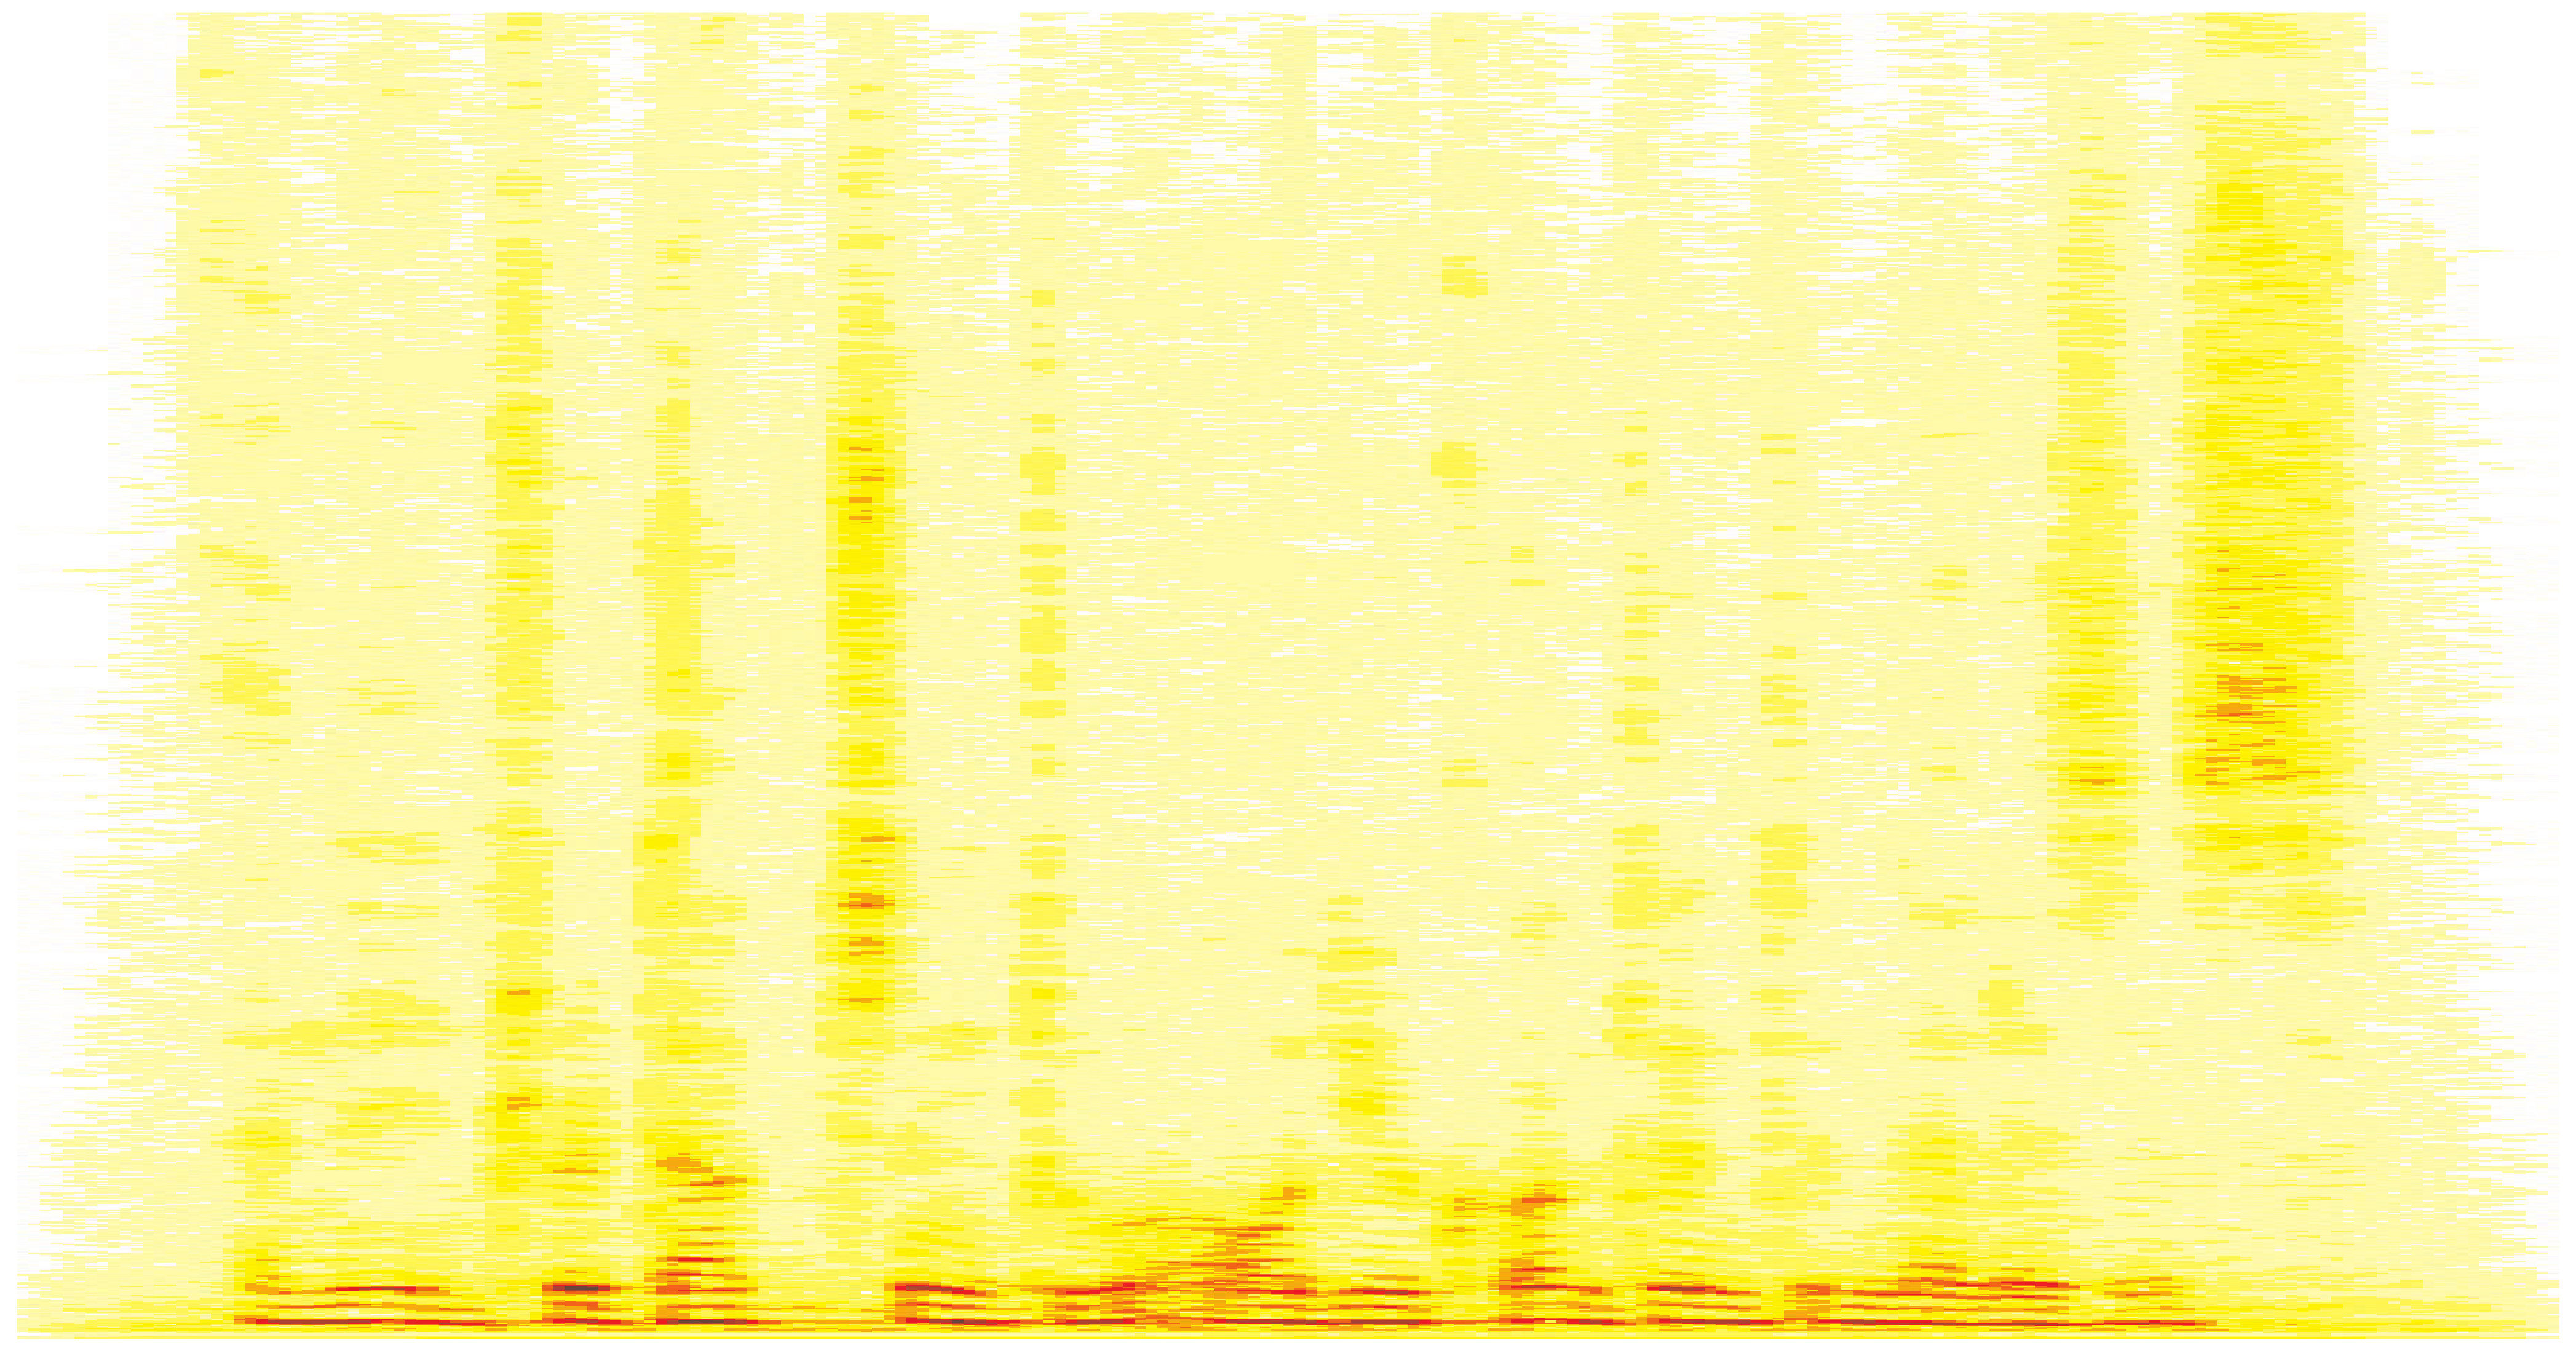
\includegraphics[width=\textwidth,height=3cm]{title}}

%%%%%%%%%%%%%%%%%%%%%%%%%%%%%%%%%%%%%%%%%%%%%%%%%%%%%%%%%%%%%%%%%%%%%%%%%%%%%%%%%%
%%%%%%%%%%%%%%%%%%%%%%%%%%%%%%%%%%%%%%%%%%%%%%%%%%%%%%%%%%%%%%%%%%%%%%%%%%%%%%%%%%
% colors
\definecolor{gtgold}{HTML}{E0AA0F} %{rgb}{0.88,0.66,1,0.06} [234, 170, 0]/256

%%%%%%%%%%%%%%%%%%%%%%%%%%%%%%%%%%%%%%%%%%%%%%%%%%%%%%%%%%%%%%%%%%%%%%%%%%%%%%%%%%
%%%%%%%%%%%%%%%%%%%%%%%%%%%%%%%%%%%%%%%%%%%%%%%%%%%%%%%%%%%%%%%%%%%%%%%%%%%%%%%%%%
% math
\DeclareMathOperator*{\argmax}{argmax}
\DeclareMathOperator*{\argmin}{argmin}
\DeclareMathOperator*{\atan}{atan}
\DeclareMathOperator*{\arcsinh}{arcsinh}
\DeclareMathOperator*{\sign}{sign}
\DeclareMathOperator*{\tcdf}{tcdf}
\DeclareMathOperator*{\si}{sinc}
\DeclareMathOperator*{\princarg}{princarg}
\DeclareMathOperator*{\arccosh}{arccosh}
\DeclareMathOperator*{\hwr}{HWR}
\DeclareMathOperator*{\flip}{flip}
\DeclareMathOperator*{\sinc}{sinc}
\DeclareMathOperator*{\floor}{floor}
\newcommand{\e}{{e}}
\newcommand{\jom}{\mathrm{j}\omega}
\newcommand{\jOm}{\mathrm{j}\Omega}
\newcommand   {\mat}[1]    		{\boldsymbol{\uppercase{#1}}}		%bold
\renewcommand {\vec}[1]    		{\boldsymbol{\lowercase{#1}}}		%bold

%%%%%%%%%%%%%%%%%%%%%%%%%%%%%%%%%%%%%%%%%%%%%%%%%%%%%%%%%%%%%%%%%%%%%%%%%%%%%%%%%%
%%%%%%%%%%%%%%%%%%%%%%%%%%%%%%%%%%%%%%%%%%%%%%%%%%%%%%%%%%%%%%%%%%%%%%%%%%%%%%%%%%
% media9
\newcommand{\includeaudio}[1]{{\includemedia[
                        addresource=audio/#1.mp3,
                        width=5mm,
                        height=5mm,
                        activate=onclick,
                        flashvars={
                            source=audio/#1.mp3  
                            &autoPlay=true
                        }]
                        {
\includegraphics[width=5mm, height=5mm]{SpeakerIcon}}
                        {APlayer.swf}}}
\newcommand{\audioautoplay}[1]{{\begin{center}\includemedia[
                            addresource=audio/#1.mp3,
                            width=.1\linewidth,
                            height=.01\linewidth,
                            activate=pageopen,
                            flashvars={
                                source=audio/#1.mp3  
                                &autoPlay=true
                            }]
                            {}
                            {APlayer.swf}\end{center}}}

\newcommand{\includevideo}[1]{{\begin{center}\includemedia[
                        addresource=video/#1.mp4,
                        width=0.8\linewidth,
                        height=0.4\linewidth,
                        activate=onclick,
                        flashvars={
                            source=video/#1.mp4  
                            &autoPlay=true
                        }]
                        {}
                        {VPlayer.swf}\end{center}}}
\newcommand{\videowithmatlab}[1]{{\begin{center}\includemedia[
                        addresource=video/animate#1.mp4,
                        width=0.8\linewidth,
                        height=0.4\linewidth,
                        activate=onclick,
                        flashvars={
                            source=video/animate#1.mp4  
                            &autoPlay=true
                        }]
                        {}
                        {VPlayer.swf}\end{center}\addreference{matlab source: matlab/animate#1.m}}}
                        

%%%%%%%%%%%%%%%%%%%%%%%%%%%%%%%%%%%%%%%%%%%%%%%%%%%%%%%%%%%%%%%%%%%%%%%%%%%%%%%%%%
%%%%%%%%%%%%%%%%%%%%%%%%%%%%%%%%%%%%%%%%%%%%%%%%%%%%%%%%%%%%%%%%%%%%%%%%%%%%%%%%%%
% other commands
\newcommand{\question}[1]{%\vspace{-4mm}
                          \setbeamercovered{invisible}
                          \begin{columns}[T]
                            \column{.8\textwidth}
                                \textbf{#1}
                            \column{.2\textwidth}
                                \vspace{-8mm}
                                \begin{flushright}
                                     
\includegraphics[scale=.5]{question_mark}
                                \end{flushright}
                                \vspace{6mm}
                          \end{columns}\pause\vspace{-12mm}}

\newcommand{\toremember}[1]{%\vspace{-4mm}
                          \begin{columns}[T]
                            \column{.8\textwidth}
                                \textbf{#1}
                            \column{.2\textwidth}
                                \vspace{-4mm}
                                \begin{flushright}
                                     
\includegraphics[scale=.5]{exclamation_mark}
                                \end{flushright}
                                \vspace{6mm}
                          \end{columns}\vspace{-6mm}}

\newcommand{\matlabexercise}[1]{%\vspace{-4mm}
                          \setbeamercovered{invisible}
                          \begin{columns}[T]
                            \column{.8\textwidth}
                                \textbf{matlab exercise}: #1
                            \column{.2\textwidth}
                                \begin{flushright}
                                     
\includegraphics[scale=.5]{logo_matlab}
                                \end{flushright}
                                %\vspace{6mm}
                          \end{columns}}

\newcommand{\addreference}[1]{  
                  
                    \begin{textblock*}{\baselineskip }(1.12\textwidth,.3\textheight) %(1.15\textwidth,.4\textheight)
                        \rotatebox{90}{\tiny {#1}}
                    \end{textblock*}}
                    
\newcommand{\figwithmatlab}[1]{
                    \begin{figure}
                        \centering
                        \includegraphics{#1}
                        %\label{fig:#1}
                    \end{figure}
                    
                    \addreference{matlab source: \href{https://github.com/alexanderlerch/ACA-Slides/blob/master/matlab/display#1.m}{matlab/display#1.m}}}
\newcommand{\figwithref}[2]{
                    \begin{figure}
                        \centering
                        \includegraphics{#1}
                        \label{fig:#1}
                    \end{figure}
                    
                    \addreference{#2}}  
                                    
\newcommand{\inserticon}[1]{

                    \begin{textblock*}{100mm}(14.5cm,7.5cm)
                        \includegraphics[height=.8cm,keepaspectratio]{#1}
                    \end{textblock*}}            

%%%%%%%%%%%%%%%%%%%%%%%%%%%%%%%%%%%%%%%%%%%%%%%%%%%%%%%%%%%%%%%%%%%%%%%%%%%%%%%%%%
%%%%%%%%%%%%%%%%%%%%%%%%%%%%%%%%%%%%%%%%%%%%%%%%%%%%%%%%%%%%%%%%%%%%%%%%%%%%%%%%%%
% counters
\newcounter{i}
\newcounter{j}
\newcounter{iXOffset}
\newcounter{iYOffset}
\newcounter{iXBlockSize}
\newcounter{iYBlockSize}
\newcounter{iYBlockSizeDiv2}
\newcounter{iDistance}



\subtitle{Module 3.1: Feature Extraction~---~Statistical Features}

%%%%%%%%%%%%%%%%%%%%%%%%%%%%%%%%%%%%%%%%%%%%%%%%%%%%%%%%%%%%%%%%%%%%%%%%%%%%
\begin{document}
    % generate title page
	

\begin{frame}
    \titlepage
    %\vspace{-5mm}
    \begin{flushright}
        \href{http://www.gtcmt.gatech.edu}{\includegraphics[height=.8cm,keepaspectratio]{logo_GTCMT_black}}
    \end{flushright}
\end{frame}


    \section[overview]{lecture overview}
        \begin{frame}{introduction}{overview}
            \begin{block}{corresponding textbook section}
                    \href{http://ieeexplore.ieee.org/xpl/articleDetails.jsp?arnumber=6331120}{Chapter 3~---~Instantaneous Features}: pp.~35--41
            \end{block}

            \begin{itemize}
                \item   \textbf{lecture content}
                    \begin{itemize}
                        \item   introduction to statistical features
                            \begin{itemize}
                                \item   mean
                                \item   variance and standard deviation
                                \item   quantiles
                            \end{itemize}
                    \end{itemize}
                \bigskip
                \item<2->   \textbf{learning objectives}
                    \begin{itemize}
                        \item   give examples of where statistical features can be used
                        \item   describe the meaning of the introduced statistical features
                    \end{itemize}
            \end{itemize}
            \inserticon{directions}
        \end{frame}

    \section[intro]{statistical features introduction}
        \begin{frame}{statistical features}{introduction}
            \begin{itemize}
                \item   statistical features are\ldots
                    \begin{itemize}
                        \item   numerical descriptors of statistical properties of the signal or its PDF
                        \item   general features that are not audio-related
                    \end{itemize}
                \smallskip
                \item   \textbf{usage}
                    \begin{itemize}
                        \item   often not directly applied to audio signal but to feature representations of it
                    \end{itemize}
            \end{itemize}
            
        \end{frame}
        
    \section[mean]{mean}
        \begin{frame}{statistical features}{arithmetic mean}
            \vspace{-7mm}
            \begin{columns}
            \column{.5\linewidth} 
            \begin{itemize}
                \item   from signal $x$:
                \vspace{-4mm}
                \begin{equation*}\label{eq:arith_mean}
                    \mu_x(n) = \frac{1}{\mathcal{K}}\sum\limits_{i=i_{\mathrm{s}}(n)}^{i_{\mathrm{e}}(n)}{x(i)} 
                \end{equation*}
                \pause
                \vspace{-4mm}
                \item   from distribution $p_x$:
                \begin{equation*}\label{eq:arith_mean2}
                    \mu_x(n) = \sum\limits_{x=-\infty}^{\infty}{x\cdot p_x(x)} 
                \end{equation*}
                \pause
                \vspace{-4mm}
                \item   from unnormalized distribution $d_x$:
                \begin{equation*}\label{eq:arith_mean3}
                    \mu_x(n) = \frac{\sum\limits_{x=-\infty}^{\infty}{x\cdot d_x(x)}}{\sum\limits_{x=-\infty}^{\infty}{d_x(x)}} 
                \end{equation*}
            \end{itemize}
            \column{.5\linewidth} 
            \vspace{-5mm}
                
            \begin{figure}
                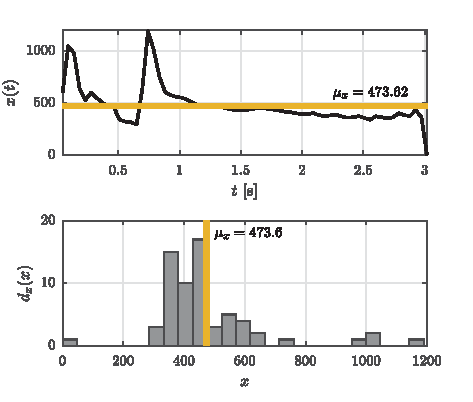
\includegraphics{Mean}
            \end{figure}
            \end{columns}
            \addreference{matlab source: \href{https://github.com/alexanderlerch/ACA-Slides/blob/master/matlab/displayMean.m}{matlab/displayMean.m}}
        \end{frame}
        \begin{frame}{statistical features}{geometric \& harmonic mean}
			\begin{itemize}
				\item	\textbf{geometric mean}
				\begin{eqnarray*}
					M_x(0,n)		&=& \sqrt[\mathcal{K}]{\prod\limits_{i=i_{\mathrm{s}}(n)}^{i_{\mathrm{e}}(n)}{x(i)}}\label{eq:geo_mean1}\\
								&=& \exp\left({\frac{1}{\mathcal{K}}\sum\limits_{i=i_{\mathrm{s}}(n)}^{i_{\mathrm{e}}(n)}{\log\big[x(i)\big]}}\right) \label{eq:geo_mean2}
				\end{eqnarray*}
                \pause
				\item	\textbf{harmonic mean}
				\begin{equation*}
					M_x(-1,n) = \frac{\mathcal{K}}{\sum\limits_{i=i_{\mathrm{s}}(n)}^{i_{\mathrm{e}}(n)}{\nicefrac{1}{x(i)}}} 
				\end{equation*}
			\end{itemize}
        \end{frame}
        \begin{frame}{statistical features}{generalized mean}
			\begin{itemize}
				\item	\textbf{generalized mean}
                    \begin{equation*}
                        M_x(\beta,n) = \sqrt[\beta]{\frac{1}{\mathcal{K}}\sum\limits_{i=i_{\mathrm{s}}(n)}^{i_{\mathrm{e}}(n)}{x^\beta(i)}} 
                    \end{equation*}
				\pause
                    \begin{footnotesize}
                    \begin{itemize}
                        \item	{$\beta=1$:} {arithmetic mean}
                        \item	{$\beta=2$:} {quadratic mean}
                        \item	{$\beta=-1$:} {harmonic mean}
                        \item	{$\beta\rightarrow 0$:} {geometric mean}
                        \item	{$\beta\rightarrow -\infty$:} {minimum}
                        \item	{$\beta\rightarrow \infty$:} {maximum}
                    \end{itemize}
                    \end{footnotesize}
			\end{itemize}
        \end{frame}
        \begin{frame}{statistical features}{statistical features~---~centroid}
			\setbeamercovered{invisible}
            \textbf{centroid}: \textit{center of gravity}
			\begin{equation*}\label{eq:centroid}
				v_{\mathrm{C}}(n) = \frac{\sum\limits_{i=i_{\mathrm{s}}(n)}^{i_{\mathrm{e}}(n)}{\big(i-i_{\mathrm{s}}(n)\big)\cdot x(i)}}{\sum\limits_{i=i_{\mathrm{s}}(n)}^{i_{\mathrm{e}}(n)}{x(i)}} 
			\end{equation*}
            
            \pause
            \question{Why does this look familiar?}
            
            $\rightarrow$ compare arithmetic mean
        \end{frame}
    \section[variance]{variance \& standard deviation}
        \begin{frame}{statistical features}{variance \& standard deviation}
            \vspace{-2mm}
			measure of \textit{spread} of the signal around its mean
            \vspace{-5mm}
            \begin{columns}
            \column{.5\linewidth} 
            \begin{itemize}
                \item \textbf{variance}
                    \begin{itemize}
                        \item   from signal block:
                        \vspace{-2mm}
                            \begin{equation*}
                                \sigma_x^2(n) = \frac{1}{\mathcal{K}}\sum\limits_{i= i_{\mathrm{s}}(n)}^{i_{\mathrm{e}}(n)}{\big(x(i)-\mu_x(n)\big)^2} 
                            \end{equation*}
                        \pause
                        \item   from distribution:
                        \vspace{-2mm}
                            \begin{equation*}
                                \sigma_x^2(n) = \sum\limits_{x=-\infty}^{\infty}{\big(x-\mu_x\big)^2\cdot p_x(x)} 
                            \end{equation*}
                    \end{itemize}
                \pause
                \item \textbf{standard deviation}
                        \vspace{-2mm}
                    \begin{equation*}
                        \sigma_x(n) = \sqrt{\sigma_x^2(n)} 
                    \end{equation*}
            \end{itemize}
            \column{.5\linewidth} 
            \vspace{-8mm}
                
            \begin{figure}
                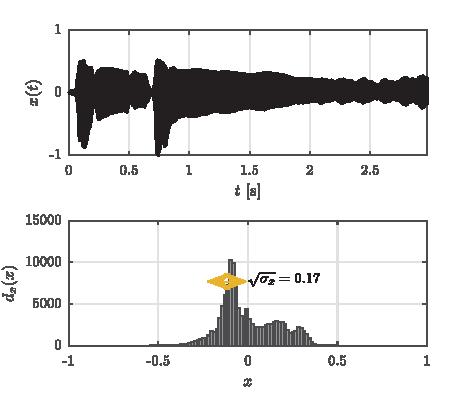
\includegraphics{Std}
            \end{figure}
            \end{columns}
            \addreference{matlab source: \href{https://github.com/alexanderlerch/ACA-Slides/blob/master/matlab/displayStd.m}{matlab/displayStd.m}}
            
        \end{frame}
        %\begin{frame}{statistical features}{statistical features~---~skewness \& kurtosis}
            %\begin{itemize}
                %\item \textbf{skewness}: measure of \textit{PDF asymmetry}
                    %\begin{equation*}
                        %v_{\mathrm{Sk}}(n) = {\frac{1}{\sigma_x^3(n)\cdot \mathcal{K}}\sum\limits_{i=i_{\mathrm{s}}(n)}^{i_{\mathrm{e}}(n)}{\left(\vphantom{\frac{1}{1}}x(i)-\mu_x(n)\right)^3}} 
                    %\end{equation*}
                    %\begin{footnotesize}
                            %\begin{itemize}
                                %\item<2->	symmetric PDFs $\rightarrow$ $0$
                                %\item<2->	left-skewed (mass center right) $\rightarrow$ negative
                                %\item<2->	right-skewed (mass center left) $\rightarrow$ positive 
                            %\end{itemize}
                    %\end{footnotesize}
                %\item<3-> \textbf{kurtosis}: measure of PDF ``\textit{Gaussianity}''
                    %\begin{equation*}
                        %v_{K}(n) = {\frac{1}{\sigma_x^4(n)\cdot \mathcal{K}}\sum\limits_{i=i_{\mathrm{s}}(n)}^{i_{\mathrm{e}}(n)}{\left(\vphantom{\frac{1}{1}}x(i)-\mu_x(n)\right)^4}} - 3 
                    %\end{equation*}
                    %\begin{footnotesize}
                            %\begin{itemize}
                                %\item<4->	Gaussian PDFs (\textit{mesokurtic})  $\rightarrow$ 0
                                %\item<4->	flat PDFs (\textit{platykurtic}) $\rightarrow$ negative
                                %\item<4->	peaky PDFs (\textit{leptokurtic})  $\rightarrow$ positive
                            %\end{itemize}	
                    %\end{footnotesize}
            %\end{itemize}
        %\end{frame}
        
    \section{quantiles}
		\begin{frame}{statistical features}{quantiles \& quantile ranges}
			dividing the PDF into (equal sized) subsets
            \vspace{-3mm}
            \begin{columns}
            \column{.4\linewidth}
            \begin{footnotesize}
			\begin{eqnarray*}
				Q_\mathrm{X}(c_p) &=& \argmin\big (F_\mathrm{X}(x) \leq c_p\big)\\
                with\quad F_\mathrm{X}(x) &=& {\int\limits_{-\infty}^{x}{p_\mathrm{x}(y)\, dy}}
			\end{eqnarray*}
            \end{footnotesize}
            \column{.6\linewidth}
            \vspace{-9mm}
			\begin{figure}
                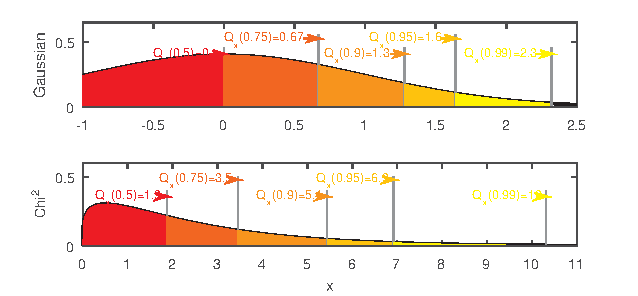
\includegraphics{PdfQuantiles}
            \end{figure}
            \end{columns}
        \end{frame}
		\begin{frame}{statistical features}{quantile examples}
			\begin{itemize}
				\item	\textbf{median}
						\begin{equation*}\label{eq:median}
							Q_\mathrm{X}(0.5) = \argmin\big (F_\mathrm{X}(x) \leq 0.5\big)
						\end{equation*}
				\bigskip
				\item	\textbf{quartiles}: $Q_\mathrm{X}(0.25),\, Q_\mathrm{X}(0.5)$, and $Q_\mathrm{X}x(0.75)$
				\bigskip
                \item	\textbf{quantile range}, e.g.
						\begin{equation*}
							\Delta Q_\mathrm{X}(0.9) = Q_\mathrm{X}(0.95)-Q_\mathrm{X}(0.05)
						\end{equation*}
			\end{itemize}
        \end{frame}
		%\begin{frame}{statistical features}{matlab exercise}
            %\matlabexercise{statistical feature implementation}
            %\begin{enumerate}
                %\item   load an audio file
                %\item   make both block size and hop size parameters of your matlab function
                %\item   implement the following features extracted per block of your time domain signal:
                    %\begin{itemize}
                        %\item   mean and median
                        %\item   variance and standard deviation
                        %\item   skewness and kurtosis
                    %\end{itemize}
            %\end{enumerate}
		%\end{frame}
        
    \section{summary}
        \begin{frame}{summary}{lecture content}
            \begin{itemize}
                \item   \textbf{statistical features}  
                    \begin{itemize}
                        \item  summarize technical signal characteristics in few numerical values 
                        \item   may be used on a time domain, frequency domain, or feature domain signal
                    \end{itemize}
                \bigskip
                \item   \textbf{feature description}
                    \begin{itemize}
                        \item   \textit{mean}: average value
                        \item   \textit{variance} and \textit{standard deviation}: measure of expected deviation from the mean
                        \item   \textit{quantiles}: numerical pdf shape description
                    \end{itemize}
            \end{itemize}
            \inserticon{summary}
        \end{frame}
\end{document}
